%-------------------------
% Resume in Latex
% Author : João Galego
% Based on: https://github.com/sb2nov/resume
% License : MIT
%
% GENERATED FILE - do not edit directly.
% Edit data/resume.json and templates/resume.tex.j2, then run scripts/build.py
%------------------------

\documentclass[letterpaper,11pt]{article}

\usepackage{latexsym}
\usepackage[empty]{fullpage}
\usepackage{titlesec}
\usepackage{marvosym}
\usepackage[usenames,dvipsnames]{color}
\usepackage{verbatim}
\usepackage{enumitem}
\usepackage{graphicx}
\usepackage[hidelinks]{hyperref}
\usepackage{fancyhdr}
\usepackage[english]{babel}
\usepackage{tabularx}
\usepackage{ragged2e}
\usepackage{fontawesome}
\usepackage[normalem]{ulem}

%----------FONT OPTIONS----------
% sans-serif
% \usepackage[sfdefault]{FiraSans}
\usepackage[sfdefault]{roboto}
% \usepackage[sfdefault]{noto-sans}
% \usepackage[default]{sourcesanspro}

% serif
% \usepackage{CormorantGaramond}
% \usepackage{charter}


\pagestyle{fancy}
\fancyhf{} % clear all header and footer fields
\fancyfoot{}
\renewcommand{\headrulewidth}{0pt}
\renewcommand{\footrulewidth}{0pt}

% Adjust margins
\addtolength{\oddsidemargin}{-0.5in}
\addtolength{\evensidemargin}{-0.5in}
\addtolength{\textwidth}{1in}
\addtolength{\topmargin}{-.5in}
\addtolength{\textheight}{1.0in}

\urlstyle{same}

\raggedbottom
\raggedright
\setlength{\footskip}{4.5pt}
\setlength{\tabcolsep}{0in}

% Sections formatting
\titleformat{\section}{
  \vspace{-4pt}\scshape\raggedright\large
}{}{0em}{}[\color{black}\titlerule \vspace{-5pt}]

%-------------------------
% Custom commands
\newcommand{\resumeItem}[1]{
  \item\small{
    {#1 \vspace{-2pt}}
  }
}

\newcommand{\resumeSubheading}[4]{
  \vspace{-2pt}\item
    \begin{tabular*}{0.97\textwidth}[t]{l@{\extracolsep{\fill}}r}
      \textbf{#1} & #2 \\
      \texttt{\small#3} & \textit{\small #4} \\
    \end{tabular*}\vspace{-7pt}
}

\newcommand{\resumeSubSubheading}[2]{
    \item
    \begin{tabular*}{0.97\textwidth}{l@{\extracolsep{\fill}}r}
      \textit{\small#1} & \textit{\small #2} \\
    \end{tabular*}\vspace{-7pt}
}

\newcommand{\resumeProjectHeading}[2]{
    \item
    \begin{tabular*}{0.97\textwidth}{l@{\extracolsep{\fill}}r}
      \small#1 & #2 \\
    \end{tabular*}\vspace{-7pt}
}

\newcommand{\resumeSubItem}[1]{\resumeItem{#1}\vspace{-4pt}}

\renewcommand\labelitemii{$\vcenter{\hbox{\tiny$\bullet$}}$}

\newcommand{\resumeSubHeadingListStart}{\begin{itemize}[leftmargin=0.15in, label={}]}
\newcommand{\resumeSubHeadingListEnd}{\end{itemize}}
\newcommand{\resumeItemListStart}{\begin{itemize}}
\newcommand{\resumeItemListEnd}{\end{itemize}\vspace{-5pt}}

\directlua{luaotfload.add_fallback
   ("emojifallback",
    {
      "NotoColorEmoji:mode=harf;"
    }
   )}

\setmainfont{texgyretermes-regular}[
  Extension      = .otf ,
  BoldFont       = texgyretermes-bold,
  ItalicFont     = texgyretermes-italic,
  BoldItalicFont = texgyretermes-bolditalic,
  RawFeature={fallback=emojifallback}
]

%-------------------------------------------

\begin{document}

\begin{center}
    \textbf{\Large \scshape CV // João Galego} \\ \vspace{1pt}
    \small
\csname faLinkedinSquare\endcsname~\href{https://www.linkedin.com/in/jgalego/}{linkedin.com/in/jgalego} $|$ \csname faGithubSquare\endcsname~\href{https://github.com/JGalego}{\texttt{github.com/JGalego}} $|$ \csname faGlobe\endcsname~\href{https://jgalego.github.io}{jgalego.github.io}\end{center}

%-----------SHORT BIO-----------

\section{Overview}

\vspace{2mm}

\justifying João Galego is Head of AI at \href{https://www.criticalsoftware.com/}{Critical Software} and Invited Professor at \href{https://iseg.ulisboa.pt}{Instituto Superior de Economia e Gestão (ISEG)}. He majored in Physics at \href{https://tecnico.ulisboa.pt/}{Instituto Superior Técnico (IST)} in Lisbon and obtained a postgraduate diploma in Forensic Studies from \href{https://www.iscsp.ulisboa.pt/}{Instituto Superior de Ciências Sociais (ISCSP)}. He did doctoral work in Cognitive Science at ULisboa, where he used machine learning (ML) to decode complex brain signals and study motor cognition. Prior to joining Critical Software, João served as Lead ML Engineer at Siemens and held roles as Solutions Architect, ML Specialist, and Quantum Ambassador at AWS. At Critical Software, his mission is to bring AI to high-stakes domains and build ML that matters. When he is not working or teaching, you can usually find him browsing local bookstores, contributing to open-source projects, or enjoying quality time with his family.


%-----------WORK EXPERIENCE-----------

\section{Professional Experience}
  \resumeSubHeadingListStart
    \vspace{2mm}
    \resumeSubheading
      {Head of AI}{2025 -- Present}
      {\href{https://www.criticalsoftware.com/}{Critical Software}}{}
    \vspace{2mm}
        \begin{itemize}
            \item Collaborate with sales and pre-sales teams to understand client requirements, support the preparation of proposals, and present AI solutions. Communicate technical concepts to nontechnical stakeholders, ensuring a clear understanding of AI projects and their impact.
            \item Oversee the end-to-end lifecycle of AI projects, from idea to production.
            \item Solution Design: Design and architect AI solutions that meet client needs and align with business goals.
            \item Engage with clients to collect requirements, conduct demos, and provide technical expertise during the sales process.
            \item Ensure that all AI solutions comply with industry regulations, ethical standards, and company policies related to the development and deployment of responsible AI.
            \item Conduct cutting-edge research on emerging AI technologies and trends, evaluating their potential impact and integration into our AI solutions to provide a competitive edge.
            \item Work with product management, engineering, data science, and other departments to deliver AI solutions that align with clients' objectives and business needs.
            \item Build and maintain partnerships with research organizations, academic institutions, and funding agencies to stay ahead of industry advancements and foster innovation opportunities.
        \end{itemize}
    \vspace{1mm}
    \resumeSubheading
      {Startup Solutions Architect}{2022 -- 2025}
      {\href{https://aws.amazon.com/}{Amazon Web Services}}{}
    \vspace{2mm}
        \begin{itemize}
            \item Work directly with strategic Startup customers to accelerate challenging, mission-critical projects
            \item Create and share best practices, technical content and new reference architectures through white papers, code samples and blog posts
            \item Evangelize and educate about AWS technology through workshops, user groups, meetups, public speaking events, online videos and conferences
            \item Collaborate within the startup ecosystem (accelerators, incubators, VCs and meetups) to educate startups and support their growth
            \item Contribute to SA organizational growth by interviewing candidates and participating in hiring decisions
            \item Member of the EMEA South Startup SA team
            \item Full member of the AI/ML Technical Field Community (TFC) focused on MLOps
            \item Full member of the AI/ML Community of Practice (CoP)
            \item GenAI Subject Matter Expert (SME) for Startups
            \item GenAI Ambassador (L200)
            \item GenAI Expert (L300+)
            \item Inclusion Ambassador
            \item AI/ML Heroes program graduate
            \item \href{https://aws.amazon.com/gameday/}{AWS GameDay} organizer, operator, maintainer and supporter
            \item AWS Senior Speaker Certified
        \end{itemize}
    \vspace{1mm}
    \resumeSubheading
      {Invited Professor}{2024 -- Present}
      {\href{https://iseg.ulisboa.pt}{ISEG / ULisboa}}{}
    \vspace{2mm}
        \begin{itemize}
            \item Lecturer for the postgraduate program in \href{https://isegexecutive.education/pt/cursos/pos-graduacoes/applied-artificial-intelligence-machine-learning/}{Applied AI/ML}
            \item Invited guest lecturer for the postgraduate program in \href{https://isegexecutive.education/pt/cursos/programas-executivos/artificial-intelligence-for-value-creation-inovar-e-desenvolver-negocios/}{AI for Value Creation}
        \end{itemize}
    \vspace{1mm}
    \resumeSubheading
      {Research Collaborator}{2020 -- Present}
      {\href{https://www.linkedin.com/company/edge-digital-lab/}{EDGE Digital Lab}}{}
    \vspace{2mm}
        \begin{itemize}
            \item The research initiative focused on the development and deployment of solutions for well-being, performance, longevity, and health based on exponential digital technologies such as AI, AR / VR, 3D printing, Blockchain, 5G, Cloud, IoT, neuroprosthetics, and more.
        \end{itemize}
    \vspace{1mm}
    \resumeSubheading
      {Lead ML Engineer}{2021 -- 2022}
      {\href{https://www.siemens.com/global/en.html}{Siemens}}{}
    \vspace{2mm}
        \begin{itemize}
            \item Member of \href{https://siemens.com/finance}{Siemens Financial Services}' Artificial Intelligence and Automation (SFS IT\&CYS AIA) chapter
            \item Development lead of robust ML solutions in an international and interdisciplinary DevOps team
            \item Senior subject-matter expert (SME) on ML technology at scale, deep learning (DL) and natural language processing (NLP)
            \item Responsible for deploying models into production while ensuring the highest standards in data integrity
            \item Responsible for implementing processes and systems for ML model lifecycle management
        \end{itemize}
    \vspace{1mm}
    \resumeSubheading
      {DevOps Engineer}{2019 -- 2021}
      {\href{https://www.siemens.com/global/en.html}{Siemens}}{}
    \vspace{2mm}
        \begin{itemize}
            \item Cloud solutions architect and administrator for 10+ applications running on AWS and Azure
            \item Lead contributor to 200+ Ansible roles, Terraform modules and Docker images
            \item Organized workshops and trainings on DevOps, AI/ML and quantum computing
            \item Performed technical assessment in 20+ interviews
            \item Supervised 10+ interns and trainees
            \item Junior member of the IT Key Experts program (Data-driven Enterprise \& Augmented Intelligence)
            \item SITEX class of 2021 working on Industrial Edge platforms and applications
            \item Member of DI IT Architecture Guild
        \end{itemize}
    \vspace{1mm}
    \resumeSubheading
      {DevOps Engineer}{2017 -- 2019}
      {\href{https://innowave.tech/}{InnoWave}}{}
    \vspace{2mm}
        \begin{itemize}
            \item Designed and implemented test frameworks and automated tests for multiple projects and customers
            \item Organized internal and customer-oriented workshops and trainings on CI/CD, DevOps and test automation
            \item Served as technical writer and reviewer working together with software architecture teams
        \end{itemize}
    \vspace{1mm}
    \resumeSubheading
      {Test Automation Engineer}{2014 -- 2017}
      {\href{https://www.coriant.com/}{Coriant}}{}
    \vspace{2mm}
        \begin{itemize}
            \item Member of the System Verification team for Optical Network Design \& Planning tools
            \item Increased test automation coverage by 5-fold in less than 2 years
            \item Managed a Jenkins cluster with 20+ build agents
        \end{itemize}
    \vspace{1mm}
  \resumeSubHeadingListEnd

%-----------EDUCATION-----------

\section{Education}
  \resumeSubHeadingListStart
    \vspace{2mm}
    \resumeSubheading
      {PhD Cognitive Science (ABD)}{2017 -- 2021}
      {\href{https://www.ulisboa.pt/}{ULisboa}}{}

        \vspace{3mm}

        Bringing minds and machines closer together using ML.

        \begin{itemize}
            \item \textbf{Title:} \textit{From Thought to Action - Machine Learning Techniques for Processing Electrophysiological Signals in Brain-Computer Interfaces}
            \item \textbf{Advisors:} \href{http://ibeb.ciencias.ulisboa.pt/pt/hugo-alexandre-ferreira/}{Prof. Hugo Ferreira} (IBEB/FCUL), \href{http://web.tecnico.ulisboa.pt/arlindo.oliveira/}{Prof. Arlindo Oliveira} (INESC/IST)
            \item \textbf{Keywords:} motor cognition, brain-computer interfaces, biosignal processing, machine learning
        \end{itemize}

        \vspace{1mm}
    \resumeSubheading
      {PgD Forensic Studies 🎓}{2016 -- 2017}
      {\href{https://www.iscsp.ulisboa.pt/}{ISCSP}}{}

        \vspace{3mm}

        Learned what "every contact leaves a trace" actually means.


        \vspace{1mm}
    \resumeSubheading
      {MSc Physics 🎓}{2008 -- 2013}
      {\href{https://tecnico.ulisboa.pt/}{IST}}{}

        \vspace{3mm}

        Failed to solve the riddle of baryon asymmetry.

        \begin{itemize}
            \item \textbf{Title:} \textit{Flavour Aspects of Multi-Higgs Models} | \textbf{Grade:} 19/20
            \item \textbf{Advisors:} Prof. Gustavo Castelo Branco (CFTP/IST)
            \item \textbf{Keywords:} standard model, CP violation, discrete groups, flavour symmetries, multi-Higgs doublet models
        \end{itemize}

        \vspace{1mm}
  \resumeSubHeadingListEnd

%-----------CERTIFICATIONS-----------

\section{Certifications}

\def\badge_height{1.4cm}
\href{https://www.credly.com/badges/be89049c-bdf4-43c9-9c54-dbc93c1fec96}{
\includegraphics[height=\badge_height]{images/aws_sa_associate.png}}
\href{https://www.credly.com/badges/db8f9c80-1b4f-4fe3-994e-038d787425be}{
\includegraphics[height=\badge_height]{images/aws_sa_professional.png}}
\href{https://www.credly.com/badges/ecbd3b46-9ab1-4b69-a0eb-5aa4fb66edd0}{
\includegraphics[height=\badge_height]{images/aws_ml_specialty.png}}
\href{https://www.credly.com/badges/1eead9ca-acd6-4ab9-b402-c2e4d2f030d5}{
\includegraphics[height=\badge_height]{images/aws_database_specialty.png}}
\href{https://www.credly.com/badges/6822536f-d65a-437c-8fed-4db09a6946dd/public\_url}{
\includegraphics[height=\badge_height]{images/aws_partner_accreditation_technical.png}}
\href{https://www.credly.com/badges/4bda2e2a-1b4c-4a02-807c-a7ebc7f712de}{
\includegraphics[height=\badge_height]{images/aws_partner_accreditation_cloud_economics.png}}
\href{https://www.credly.com/org/amazon-web-services/badge/migration-ambassador-foundations-business-2022}{
\includegraphics[height=\badge_height]{images/aws_migration_ambassador_foundations_2022_business.png}}
\href{https://www.credly.com/badges/ecbd3b46-9ab1-4b69-a0eb-5aa4fb66edd0}{
\includegraphics[height=\badge_height]{images/google_certs_da.png}}
\href{https://developers.google.com/certification/associate-android-developer}{
\includegraphics[height=\badge_height]{images/certified_android_developer.png}}
\href{https://www.credly.com/badges/8b9deb9d-34be-4ae5-b76c-b76cc2ec8381}{
\includegraphics[height=\badge_height]{images/azure_fundamentals.png}}
\href{https://www.credly.com/badges/ce2d880c-1faf-4047-bc91-d3cd5d60a8eb}{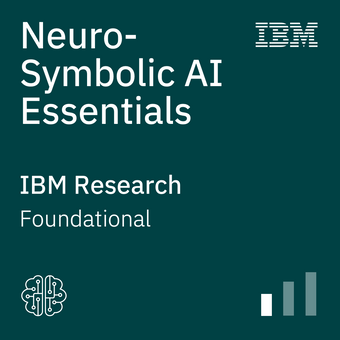
\includegraphics[height=\badge_height]{images/ibm_neuro_symbolic_ai_essentials.png}}
\href{https://www.credly.com/badges/16334ec2-f99f-4370-803e-ae8e4ea94a98}{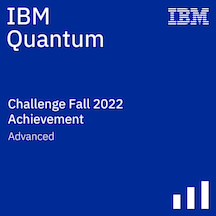
\includegraphics[height=\badge_height]{images/ibm_quantum_challenge_fall_2022.png}}
\href{https://www.credly.com/badges/9e2e2bae-d10d-4e3a-aa13-e95a35e8f8c3}{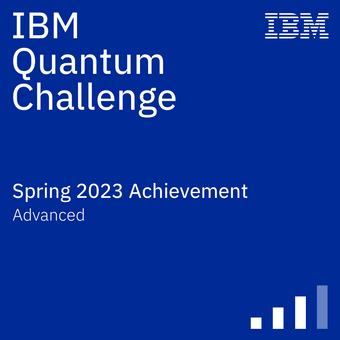
\includegraphics[height=\badge_height]{images/ibm_quantum_challenge_spring_2023.png}}

\resumeSubHeadingListStart
    \vspace{2mm}
    \resumeSubheading
      {\href{https://www.oxfordml.school/}{Oxford Machine Learning Summer School - AI for Global Goals}}{2025}
      {AI for Global Goals}{}
    \vspace{2mm}

    ML summer school with dedicated tracks for ML x Health \& Bio and ML x Rep. Learning \& GenAI organised by \href{https://www.globalgoals.ai/}{AI for Global Goals} in partnership with the \href{https://www.oxfordmartin.ox.ac.uk/deep-medicine/}{University of Oxford's Deep Medicine} and \href{https://cifar.ca/}{CIFAR} and sponsored by \href{https://www.deepmind.com/}{DeepMind}, \href{https://www.janestreet.com/}{Jane Street} and \href{https://www.gresearch.com/}{G-Research}.

    \vspace{2mm}
    \resumeSubheading
      {\href{https://luma.com/pqzv80yd}{Neuro-Symbolic AI Summer School}}{2025}
      {Centaur AI Institute}{}
    \vspace{2mm}

    A free, fully-remote, two-day event that aims to accelerate progress in the fast-emerging area of neuro-symbolic AI by teaching graduate students, data scientists, and researchers principles from the side of AI they may be less familiar with, as well as presenting a curation of emerging research ideas at the intersection. The 4$^{th}$ edition theme was "AI for Precise Computation: Mathematics, Reasoning, and Planning".

    \vspace{2mm}
    \resumeSubheading
      {\href{https://www.oxfordml.school/}{Oxford Machine Learning Summer School - AI for Global Goals}}{2024}
      {AI for Global Goals}{}
    \vspace{2mm}

    ML summer school with dedicated tracks for ML x Health \& Bio and ML x Rep. Learning \& GenAI organised by \href{https://www.globalgoals.ai/}{AI for Global Goals} in partnership with the \href{https://www.oxfordmartin.ox.ac.uk/deep-medicine/}{University of Oxford's Deep Medicine} and \href{https://cifar.ca/}{CIFAR} and sponsored by \href{https://www.deepmind.com/}{DeepMind} and \href{https://www.gsk.ai/}{GSK}.

    \vspace{2mm}
    \resumeSubheading
      {\href{https://aws.amazon.com/certification/certified-solutions-architect-associate/}{AWS Certified Solutions Architect - Professional}}{2024}
      {Amazon}{}
    \vspace{2mm}

    Professional-level exam intended for individuals with two or more years of hands-on experience designing and deploying cloud architecture on AWS.

    \vspace{2mm}
    \resumeSubheading
      {\href{https://aws.amazon.com/certification/certified-machine-learning-specialty/}{AWS Certified Database - Specialty}}{2023}
      {Amazon}{}
    \vspace{2mm}

    Specialty-level exam to assess the candidate's comprehensive understanding of databases, including the concepts of design, migration, deployment, access, maintenance, automation, monitoring, security, and troubleshooting.

    \vspace{2mm}
    \resumeSubheading
      {\href{https://www.oxfordml.school/}{Oxford Machine Learning Summer School - AI for Global Goals}}{2022}
      {AI for Global Goals}{}
    \vspace{2mm}

    ML summer school with dedicated tracks for ML x Finance and ML x Health organised by \href{https://www.globalgoals.ai/}{AI for Global Goals} in partnership with the \href{https://www.oxfordmartin.ox.ac.uk/deep-medicine/}{University of Oxford's Deep Medicine} and \href{https://cifar.ca/}{CIFAR} and sponsored by \href{https://www.deepmind.com/}{DeepMind} and \href{https://www.gsk.ai/}{GSK}.

    \vspace{2mm}
    \resumeSubheading
      {\href{http://startupschool.org/}{Startup School}}{2022}
      {Y Combinator}{}
    \vspace{2mm}

    7-week course featuring live talks by YC partners, founder stories by YC alumni, in-person meetups at YC offices all over the world, co-founder matching, and the largest community of startup founders on the internet cf. \href{https://www.ycombinator.com/blog/announcing-startup-school-2022}{Announcing Startup School 2022} for the official announcement.

    \vspace{2mm}
    \resumeSubheading
      {\href{https://aws.amazon.com/certification/certified-solutions-architect-associate/}{AWS Certified Solutions Architect - Associate}}{2022}
      {Amazon}{}
    \vspace{2mm}

    Associate-level exam to assess the candidate's ability to design and build secure, high-performing, cost-effective, highly available, and scalable solutions based on customer requirements.

    \vspace{2mm}
    \resumeSubheading
      {\href{https://explore.skillbuilder.aws/learn/course/12350/Migration\%2520Ambassador\%2520Foundations\%2520\%28Business\%29}{Migration Ambassador Foundations (Business)}}{2022}
      {Amazon}{}
    \vspace{2mm}

    Earners of this badge are individuals who have demonstrated the foundational business knowledge about AWS Cloud Migration and the AWS Programs to support a customer's migration to the AWS Cloud.

    \vspace{2mm}
    \resumeSubheading
      {\href{https://aws.amazon.com/partners/training/accreditation/}{AWS Partner: Accreditation (Technical)}}{2022}
      {Amazon}{}
    \vspace{2mm}

    This accreditation provides \href{https://aws.amazon.com/partners/}{AWS Partners} with fundamental, technical knowledge of AWS cloud computing, global infrastructure, services, common solutions, migration, security, and compliance.

    \vspace{2mm}
    \resumeSubheading
      {\href{https://aws.amazon.com/partners/training/accreditation/}{AWS Partner: Cloud Economics Accreditation}}{2022}
      {Amazon}{}
    \vspace{2mm}

    Earners of this badge are \href{https://aws.amazon.com/partners/}{AWS Partners} who have demonstrated knowledge of cost savings and data center economics in relation to \href{https://aws.amazon.com/economics/}{cloud computing}.

    \vspace{2mm}
    \resumeSubheading
      {\href{https://www.coursera.org/specializations/machine-learning-engineering-for-production-mlops}{Machine Learning Engineering for Production (MLOps) Specialization}}{2021}
      {DeepLearning.AI}{}
    \vspace{2mm}

    Multi-course specialization on how to \textit{productionize} ML applications, organized in collaboration with \href{https://www.deeplearning.ai/}{DeepLearning.AI} and the Google \href{https://www.tensorflow.org/}{TensorFlow} team.

    \vspace{2mm}
    \resumeSubheading
      {\href{https://www.coursera.org/specializations/natural-language-processing}{Natural Language Processing (NLP) Specialization}}{2021}
      {DeepLearning.AI}{}
    \vspace{2mm}

    Multi-course specialization on how to design NLP applications that perform such tasks as sentiment analysis and language translation, organized in collaboration with \href{https://www.deeplearning.ai/}{DeepLearning.AI} and the Google \href{https://www.tensorflow.org/}{TensorFlow} team.

    \vspace{2mm}
    \resumeSubheading
      {\href{https://grow.google/dataanalytics}{Google Data Analytics Professional Certificate}}{2021}
      {Google}{}
    \vspace{2mm}

    Multi-course certificate program on how to collect, transform, and organize of data in order to draw conclusions, make predictions, and drive informed decision-making.

    \vspace{2mm}
    \resumeSubheading
      {\href{https://www.udacity.com/course/ai-product-manager-nanodegree--nd088}{AI Product Manager Nanodegree}}{2021}
      {Udacity}{}
    \vspace{2mm}

    Course on how to develop AI products that deliver business value, organized in collaboration with \href{https://appen.com/}{Appen}.

    \vspace{2mm}
    \resumeSubheading
      {\href{https://www.udacity.com/course/self-driving-car-engineer-nanodegree--nd013}{Self-Driving Car Engineer Nanodegree}}{2021}
      {Udacity}{}
    \vspace{2mm}

    Autonomous driving course covering several topics in computer vision, sensor fusion, localization, path planning, control and systems integration, organized in collaboration with \href{https://waymo.com/}{Waymo} and \href{https://www.mercedes-benz.com/en/innovation/autonomous/}{Mercedes-Benz}.

    \vspace{2mm}
    \resumeSubheading
      {\href{https://aws.amazon.com/certification/certified-machine-learning-specialty/}{AWS Certified Machine Learning - Specialty}}{2020}
      {Amazon}{}
    \vspace{2mm}

    Specialty-level exam to assess the candidate's ability to design, implement, deploy, and maintain ML solutions.

    \vspace{2mm}
    \resumeSubheading
      {\href{https://learndigital.withgoogle.com/digitalgarage/course/digital-marketing}{Fundamentals of Digital Marketing}}{2020}
      {Google}{}
    \vspace{2mm}

    Intro to digital marketing course accredited by \href{https://iabeurope.eu/0}{Interactive Advertising Bureau Europe} and \href{https://www.open.ac.uk/}{The Open University}.

    \vspace{2mm}
    \resumeSubheading
      {\href{https://docs.microsoft.com/en-us/learn/certifications/azure-fundamentals/}{Microsoft Certified Azure Fundamentals (AZ-900)}}{2020}
      {Microsoft}{}
    \vspace{2mm}

    Azure certification covering fundamental cloud concepts, Azure services, Azure workloads, security and privacy in Azure, as well as Azure pricing and support.

    \vspace{2mm}
    \resumeSubheading
      {\href{https://developers.google.com/certification/associate-android-developer}{Associate Android Developer}}{2018}
      {Google}{}
    \vspace{2mm}

    Entry-level exam that includes a coding project and exit interview, covering topics related to app functionality, UI and data management, as well as debugging and testing of Android apps.

    \vspace{2mm}
    \resumeSubheading
      {\href{https://www.cloudbees.com/jenkins/certification}{Certified Jenkins Engineer}}{2016}
      {Cloudbees}{}
    \vspace{2mm}

    Official certification covering core \href{https://www.cloudbees.com/jenkins/what-is-jenkins}{Jenkins} concepts, Pipeline and Jenkins administration fundamentals.

    \vspace{2mm}
    \resumeSubheading
      {\href{https://www.coursera.org/learn/machine-learning}{Machine Learning}}{2014}
      {Coursera}{}
    \vspace{2mm}

    Introductory MOOC on machine learning taught by \href{https://www.andrewng.org/}{Andrew Ng}.

    \vspace{2mm}
\resumeSubHeadingListEnd

%-----------TECHNICAL SKILLS-----------

\section{Technical Skills}

\vspace{2mm}

{\small\textbf{Disclaimer:} \emph{This list is neither extensive nor exhaustive by design. As a firm believer in the "right tool for the right job" mindset, I've had the chance to work with hundreds of tools, packages and frameworks throughout my career. Listing them all here would be cumbersome and, worse, uninformative. Please contact me directly if you wish to discuss specific technical skills.}}

\begin{itemize}[leftmargin=0.15in, label={}]

    \item Hands-on experience with multiple cloud providers (AWS, Azure, Google Cloud).

    \item Active contributor to several open source projects:

    \begin{itemize}
        \item \textbf{\href{https://github.com/aws-samples}{AWS Samples}} - Bedrock Access Gateway
        \item \textbf{\href{https://github.com/awslabs}{AWS Labs}} - Project Lakechain
        \item \textbf{\href{https://github.com/google-deepmind}{Google DeepMind}} - Concordia
        \item \textbf{\href{https://github.com/huggingface/}{Hugging Face}} - Text Embedding Inference (TEI)
        \item \textbf{\href{https://github.com/langchain-ai/langchain}{LangChain}} - LangChain, LangServe
        \item \textbf{\href{https://github.com/nus-apr}{APR@NUS}} - AutoCodeRover
        \item \textbf{\href{https://github.com/princeton-nlp/}{Princeton NLP}} - SWE-Agent
        \item \textbf{\href{https://github.com/ScrapeGraphAI/}{ScrapeGraphAI}} - Scrapegraph-ai
        \item \textbf{\href{https://github.com/stanfordnlp/}{Stanford NLP}} - DSPy
        \item \textbf{\href{https://github.com/OpenGenerativeAI}{OpenGenerativeAI}} - LLM Colosseum
        \item \textbf{\href{https://github.com/declare-lab}{DeCLaRe Lab}} - LLM PuzzleTest
        \item \textbf{\href{https://github.com/aurelio-labs}{Aurelio AI Labs}} - Semantic Router
    \end{itemize}

    \item Working knowledge of multiple programming and scripting languages:

    \begin{itemize}
        \item \textbf{Proficient} - Java, Python
        \item \textbf{Professional Use} - C++, C\#, Dart (Flutter), Go, Groovy, JavaScript, Lua, MATLAB, Ruby, Rust
        \item \textbf{Academic Use} - C, Coq, Haskell, Lean, Lisp, Prolog, R, Wolfram Mathematica
    \end{itemize}

    \item Expert knowledge of multiple DevOps tools:

    \begin{itemize}
        \item \textbf{Automation} - Ansible, Packer, Terraform, Vagrant
        \item \textbf{CI/CD} - Azure DevOps, GitLab CI, Jenkins
        \item \textbf{Containerization} - Docker, Kubernetes
        \item \textbf{Logging \& Monitoring} - Elastic (ELK) Stack, Grafana
        \item \textbf{Package Management} - JFrog Artifactory
        \item \textbf{Secrets Management} - HashiCorp Vault
        \item \textbf{Virtualization} - VirtualBox, VMware
    \end{itemize}

    \item NumPy, SciPy, Pandas, Vaex, JAX, MXNet, PyTorch, TensorFlow, Gensim, NLTK, spaCy, TextBlob, HuggingFace Transformers, HuggingFace Diffusers, Keras, Scikit-Learn, Trax.

    \item Expert knowledge of data and ML engineering tools and frameworks:

    \begin{itemize}
        \item \textbf{AutoML} - AutoGluon, AutoKeras, NNI
        \item \textbf{Data \& Model Versioning} - DVC, Git-LFS
        \item \textbf{Data Exploration} - JupyterLab, Jupyter Notebook
        \item \textbf{Data Processing} - Airflow, Hadoop, Spark 2.x, Spark 3.x
        \item \textbf{Data Visualization} - Bokeh, Dash, Facets
        \item \textbf{Feature Storage} - Amazon SageMaker Feature Store, Feast
        \item \textbf{Hyperparameter Tuning} - Scikit-Optimize, Talos, Tune
        \item \textbf{ML Platforms} - Dataiku, Kubeflow, TFX
        \item \textbf{Model Interpretability} - Alibi, Lucid
        \item \textbf{Model Lifecycle} - MLflow
        \item \textbf{Model Serialisation} - ONNX
        \item \textbf{Model Serving} - TensorFlow Serving, TorchServe, Triton Inference Server
        \item \textbf{Model Monitoring} - Evidently, Neptune
        \item \textbf{Optimization Tools} - Dask, Mahout
        \item \textbf{Simplification Tools} - Hermione, Ludwig
        \item \textbf{Visual Analysis and Debugging} - Manifold, Netron, Yellowbrick
    \end{itemize}
\end{itemize}

%-----------HONORS & AWARDS-----------

\section{Honors \& Awards}
  \resumeSubHeadingListStart
    \vspace{2mm}
    \resumeSubheading
      {\href{https://qiskit.org/events/summer-school/}{IBM QGSS25 Certificate of Quantum Excellence}}{2025}
      {IBM}{}
    \vspace{3mm}

    Two-week intensive quantum computing summer school organized by the \href{https://qiskit.org/}{IBM Qiskit} team with a focus on the \href{https://quantum2025.org/}{past, present and future of quantum computing}. Quantum excellence certificates were issued to those who completed \textit{all} graded lab work assignments. For more information, check out the \href{https://www.ibm.com/quantum/blog/qiskit-summer-school-2025}{official announcement} on the IBM research blog.
    \vspace{2mm}
    \resumeSubheading
      {EMEA CS SA GenAI Builders Quest - 1$^{st}$ Place, GenAI Trailblazers}{2023}
      {AWS}{}
    \vspace{3mm}

    Internal competition aimed to encourage SAs in EMEA CS to deepen their GenAI domain knowledge (L200+), supporting field readiness to guide customers with prescriptive guidance, advanced customer conversations, and earn their trust.
    \vspace{2mm}
    \resumeSubheading
      {\href{https://research.ibm.com/blog/quantum-challenge-spring-2023}{IBM Quantum Challenge - Advanced, 1$^{st}$ Place}}{2023}
      {IBM}{}
    \vspace{3mm}

    Quantum computing hackathon organized by \href{https://quantum-computing.ibm.com/}{IBM Quantum} dedicated to \href{https://quantum-computing.ibm.com/services/programs/docs/runtime/manage/systems/dynamic-circuits/Introduction-To-Dynamic-Circuits}{dynamic circuits}. For more information, check out the \href{https://research.ibm.com/blog/quantum-challenge-spring-2023}{official announcement} on the IBM research blog.
    \vspace{2mm}
    \resumeSubheading
      {\href{https://simoninithomas.github.io/deep-rl-course/}{Hugging Face 🤗 Deep Reinforcement Learning Course - Certificate of Excellence}}{2023}
      {Hugging Face}{}
    \vspace{3mm}

    Online course organized by \href{https://huggingface.co/}{Hugging Face} covering beginner- to expert-level topics on Deep RL. Certificates of excellence were issued to all participants that passed \textbf{all} assignments before the end of April 2023. For more information, check out the \href{https://huggingface.co/blog/deep-rl-intro}{official announcement} on the Hugging Face 🤗 blog.
    \vspace{2mm}
    \resumeSubheading
      {\href{https://research.ibm.com/blog/quantum-challenge-fall-2022}{IBM Quantum Challenge - Advanced, 1$^{st}$ Place}}{2022}
      {IBM}{}
    \vspace{3mm}

    Space-themed, quantum computing hackathon organized by \href{https://quantum-computing.ibm.com/}{IBM Quantum}. Exercises included an exploration of primitives using the new \href{https://qiskit.org/documentation/partners/qiskit\_ibm\_runtime/}{Qiskit Runtime}, applying error mitigation techniques like \href{https://github.com/Qiskit-Partners/mthree}{matrix-free measurement mitigation} (M3) to ML problems involving quantum kernels, implementing \href{https://arxiv.org/abs/2006.05643}{problem-specific parameterized quantum circuits} to solve the traveling salesman problem, and the application of quantum chemistry techniques to study the \href{https://pubs.rsc.org/en/content/chapterhtml/2017/bk9781782627760-00001?isbn=978-1-78262-776-0}{interstellar medium} by computing the reaction energy of H₃⁺, the first \href{https://arxiv.org/abs/1805.08138}{excited state} and dipole moment of C₃H₂ (\href{https://pubmed.ncbi.nlm.nih.gov/11542419/}{Cyclopropenylidene}), and the interstellar chain reaction energy of \href{https://pubs.acs.org/doi/10.1021/jp020310z}{C + C₂H₂ → C₃H₂}. For more information, check out the \href{https://research.ibm.com/blog/quantum-challenge-fall-2022}{official announcement} on the IBM research blog.
    \vspace{2mm}
    \resumeSubheading
      {Machine Learning University - AutoGluon - Top 10}{2022}
      {AWS}{}
    \vspace{3mm}

    Internal \href{https://auto.gluon.ai/stable/index.html}{AutoGluon} competition promoted by \href{https://aws.amazon.com/machine-learning/mlu/}{Machine Learning University} (MLU) as part of the \textit{AutoGluon: Beyond the Basics} workshop - the goal was to create a model for binary classification on a multimodal setting (image, text, and tabular data).
    \vspace{2mm}
    \resumeSubheading
      {Machine Learning University - GML - Top 10}{2022}
      {AWS}{}
    \vspace{3mm}

    Internal \href{https://web.stanford.edu/class/cs224w/}{graph machine learning} (GML) competition promoted by \href{https://aws.amazon.com/machine-learning/mlu/}{Machine Learning University} (MLU) as part of the accelerated GML track - the goal was to create a model to identify whether a chemical compound (represented as a graph) is \texttt{mutagenic} in nature or not cf. \href{https://paperswithcode.com/sota/graph-classification-on-mutag}{graph classification on MUTAG} for additional information.
    \vspace{2mm}
    \resumeSubheading
      {\href{https://qhack.ai/}{QHack 2022 QML Challenge - Top 70 (*)}}{2022}
      {Xanadu}{}
    \vspace{3mm}

    Quantum machine learning hackathon hosted by \href{https://www.xanadu.ai/}{Xanadu} and multiple sponsors. Won 400\$ in credits for AWS and access to an \href{https://www.ibm.com/quantum-computing/systems/}{IBM Quantum}'s 7-qubit device. (*) Due to conflicting engagements, participation in the Coding Challenge was only active during the 1$^{st}$ week.
    \vspace{2mm}
    \resumeSubheading
      {\href{https://qiskit.org/events/summer-school/}{IBM QGSS21 Certificate of Quantum Excellence}}{2021}
      {IBM}{}
    \vspace{3mm}

    Two-week intensive quantum computing summer school organized by the \href{https://qiskit.org/}{IBM Qiskit} team with a focus on \href{https://medium.com/qiskit/introducing-qiskit-machine-learning-5f06b6597526}{quantum machine learning}. Quantum excellence certificates were issued to those who completed \textit{all} graded lab work assignments with a final cumulative score above 75\%. For more information, check out the \href{https://research.ibm.com/blog/qiskit-summer-school-machine-learning}{official announcement} on the IBM research blog.
    \vspace{2mm}
    \resumeSubheading
      {Google Cloud Hero: BigQuery - Analytics \& Machine Learning - 1$^{st}$ Place}{2021}
      {Google / Siemens}{}
    \vspace{3mm}

    Invite-only event organized by \href{https://cloud.google.com/}{Google Cloud} and hosted by the Google Siemens Account team. Google Cloud Hero is a \textit{gamified} 3h training experience using hands-on labs focused on \href{https://cloud.google.com/bigquery}{BigQuery} and \href{https://cloud.google.com/bigquery-ml/docs}{BigQuery ML}.
    \vspace{2mm}
    \resumeSubheading
      {\href{https://research.ibm.com/blog/quantum-challenge-2021}{IBM Quantum Challenge - Advanced, 1$^{st}$ Place}}{2021}
      {IBM}{}
    \vspace{3mm}

    Quantum computing hackathon organized by IBM to celebrate the 40-year anniversary of the \textit{Physics of Computation} conference, and 5-year anniversary of \href{https://quantum-computing.ibm.com/}{IBM Quantum}. Exercises included factoring small integers with Shor's algorithm, running spectroscopy experiments against \textit{real} IBM Quantum systems (w/ exclusive access to the brand new \texttt{IBMQ Jakarta}) using \href{https://qiskit.org/documentation/apidoc/pulse.html}{Qiskit Pulse} and determining the ground state energy of small molecules (H₂, LiH) using \href{https://qiskit.org/textbook/ch-applications/vqe-molecules.html}{VQE}. For more information, check out the \href{https://research.ibm.com/blog/quantum-challenge-2021}{official announcement} on the IBM research blog.
    \vspace{2mm}
    \resumeSubheading
      {\href{https://www.udacity.com/bertelsmann-tech-scholarships}{Udacity Technology Scholarship - AI Track}}{2021}
      {Udacity / Bertelsmann}{}
    \vspace{3mm}

    Full scholarship to attend Udacity's \href{https://www.udacity.com/course/ai-product-manager-nanodegree--nd088}{AI Product Manager} nanodegree. See also the \href{https://sites.google.com/udacity.com/bertelsmann-tech-scholarship/ai-track}{AI Track}.
    \vspace{2mm}
    \resumeSubheading
      {\href{https://github.com/XanaduAI/QHack2021}{QHack 2021 QML Challenge - Top 50}}{2021}
      {Xanadu / AWS}{}
    \vspace{3mm}

    Quantum machine learning hackathon hosted by \href{https://aws.amazon.com/}{AWS} and \href{https://www.xanadu.ai/}{Xanadu}. Won 250\$ in credits for AWS and early access to an alpha version of Sandbox@Alphabet's \href{https://venturebeat.com/2021/03/10/alphabet-is-repurposing-google-tpus-for-quantum-computing-simulations/}{Floq simulator} 🦜 - a quantum SaaS API built on top of TPUs. For more information, read my \textit{[QHack Recap - PennyLane, Amazon Braket and Beyond](https://medium.com/@joao.galego/qhack-recap-pennylane-amazon-braket-and-beyond-a2c153d50a88)} article on Medium.
    \vspace{2mm}
    \resumeSubheading
      {SITEX 2021 - Industrial Edge, 1$^{st}$ Place}{2021}
      {Siemens}{}
    \vspace{3mm}

    Created an application that brings simulation (\href{https://www.plm.automation.siemens.com/global/en/products/manufacturing-planning/plant-simulation-throughput-optimization.html}{Tecnomatix® PlantSim}) and optimization (\href{https://www.plm.automation.siemens.com/global/pt/products/simcenter/simcenter-heeds.html}{Simcenter HEEDS}) to the factory floor 🏭 and low code platforms (\href{https://www.mendix.com/}{Mendix}) to the \href{https://new.siemens.com/global/en/products/automation/topic-areas/industrial-edge.html}{Industrial Edge} landscape as part of a strategic development program for the innovation and technology community in the Siemens hemisphere.
    \vspace{2mm}
    \resumeSubheading
      {\href{https://ecosystem.siemens.com/ai-hackathon}{AI@Sustainability Hackathon - Technical Excellence (Team Mobility)}}{2020}
      {Siemens}{}
    \vspace{3mm}

    Built an application based on \href{https://aws.amazon.com/sagemaker/}{Amazon SageMaker} in collaboration with \href{https://www.sbb.ch/}{*Swiss Federal Railways* (SBB)} 🚂 to predict the \textit{traffic volume} and \textit{modal split} for a specific weather constellation and time based on a large set of real-world data points.
    \vspace{2mm}
    \resumeSubheading
      {Associate Android Developer Fast Track Program Scholarship}{2016}
      {Google / Udacity}{}
    \vspace{3mm}

    Full scholarship to attend Udacity's fast track course and take the \href{https://developers.google.com/certification/associate-android-developer}{Associate Android Developer} exam.
    \vspace{2mm}
    \resumeSubheading
      {Junior Research Scholarship}{2013}
      {Fundação para a Ciência e Tecnologia (FCT)}{}
    \vspace{3mm}

    Scholarship for undergraduate students to work at the \href{http://cftp.ist.utl.pt/}{*Center for Theoretical Particle Physics* (CFTP)}.
    \vspace{2mm}
  \resumeSubHeadingListEnd

%-----------ARTICLES & BLOGS-----------

\section{Articles \& Blogs}
  \resumeSubHeadingListStart
    \vspace{2mm}
    \resumeSubheading
      {\href{https://community.aws/content/2j0H7GskVBBq4UJznR0GEtVIeV8/everything-s-a-graph-hacking-graphrag-with-amazon-bedrock}{Hacking GraphRAG with Amazon Bedrock}}{2024}
      {AWS Community}{}
    \vspace{3mm}

    Learn how to run GraphRAG pipelines backed by Amazon Bedrock using LiteLLM proxy.

    \vspace{2mm}
    \resumeSubheading
      {\href{https://community.aws/content/2im2sOOlZMSY5rCz2qZ1We3OPna/make-programs-not-prompts-dspy-pipelines-with-llama-3-on-amazon-sagemaker-jumpstart}{Make Programs, not Prompts: DSPy Pipelines with Llama 3 on Amazon SageMaker JumpStart}}{2024}
      {AWS Community}{}
    \vspace{3mm}

    Learn how to create ML pipelines with DSPy powered by Meta's Llama 3 70B Instruct model running on Amazon SageMaker.

    \vspace{2mm}
    \resumeSubheading
      {\href{https://community.aws/content/2ie755wmzuBOKCEu2YehiWE2dOA/leaving-no-language-behind-with-amazon-sagemaker-serverless-inference}{Leaving no language behind with Amazon SageMaker Serverless Inference}}{2024}
      {AWS Community}{}
    \vspace{3mm}

    Host a high-quality translation model at scale using Amazon SageMaker Serverless Inference.

    \vspace{2mm}
    \resumeSubheading
      {\href{https://community.aws/content/2hXqq9IE65WzyrfvqM57Za0lEgF/build-document-processing-pipelines-with-project-lakechain}{Build Document Processing Pipelines with Project Lakechain}}{2024}
      {AWS Community}{}
    \vspace{3mm}

    Learn how to create cloud-native, AI-powered document processing pipelines on AWS with Project Lakechain.

    \vspace{2mm}
    \resumeSubheading
      {\href{https://community.aws/content/2gYNfgF0VRkzU9tDmg23vCEC2BH/your-idea-is-my-command-multi-agent-collaboration-for-software-development}{Your idea is my command: multi-agent collaboration for software development}}{2024}
      {AWS Community}{}
    \vspace{3mm}

    Create your own virtual software company with Amazon Bedrock and ChatDev and use it to build custom applications through LLM-powered multi-agent interactions.

    \vspace{2mm}
    \resumeSubheading
      {\href{https://community.aws/content/2grhh3vrinYLsg3xkFNCe4LCcUL/running-langchain-js-applications-on-aws-lambda}{Running LangChain.js Applications on AWS Lambda}}{2024}
      {AWS Community}{}
    \vspace{3mm}

    Learn how to run LangChain.js apps powered by Amazon Bedrock on AWS Lambda using function URLs and response streaming.

    \vspace{2mm}
    \resumeSubheading
      {\href{https://community.aws/content/2gjRWwp4Eb51SXt6FRZNxVh71R7/scrape-all-things-ai-powered-web-scraping-with-scrapegraphai-and-amazon-bedrock}{Scrape All Things: AI-powered web scraping with ScrapeGraphAI and Amazon Bedrock}}{2024}
      {AWS Community}{}
    \vspace{3mm}

    Learn how to extract information from documents and websites using natural language prompts.

    \vspace{2mm}
    \resumeSubheading
      {\href{https://community.aws/content/2g5J4RT6lli2jetVcHezTRpKZFu/bug-hunting-with-amazon-bedrock-and-swe-agent}{Bug hunting with Amazon Bedrock and SWE-Agent}}{2024}
      {AWS Community}{}
    \vspace{3mm}

    Use Amazon Bedrock with SWE-Agent to create your own software engineering agent that can fix real-life bugs and issues in GitHub repositories.

    \vspace{2mm}
    \resumeSubheading
      {\href{https://community.aws/content/2fTJuxaxuSwl64cVakqtuEK4tnl/running-small-language-models-on-aws-lambda}{Fighting Hallucinations with LLM Cascades}}{2024}
      {AWS Community}{}
    \vspace{3mm}

    Learn how to implement FrugalGPT-style LLM cascades on top of Amazon Bedrock using LangChain and LangGraph without breaking the bank.

    \vspace{2mm}
    \resumeSubheading
      {\href{https://community.aws/content/2fTJuxaxuSwl64cVakqtuEK4tnl/running-small-language-models-on-aws-lambda}{Running Small Language Models on AWS Lambda}}{2024}
      {AWS Community}{}
    \vspace{3mm}

    Learn how to run small language models (SLMs) at scale on AWS Lambda with function URLs and response streaming.

    \vspace{2mm}
    \resumeSubheading
      {\href{https://community.aws/content/2eoCtgociSBhGfirRM0Tk0PSgxH/mapping-embeddings-from-meaning-to-vectors-and-back}{Mapping embeddings: from meaning to vectors and back}}{2024}
      {AWS Community}{}
    \vspace{3mm}

    My adventures with RAGmap and RAGxplorer with a light introduction to embeddings, vector databases, dimensionality reduction and advanced retrieval mechanisms.

    \vspace{2mm}
    \resumeSubheading
      {\href{https://community.aws/content/2evcvfrOpxaXTIv3uPchFaKKjAf/tgifun-building-genai-apps-with-managed-ai-services}{Building GenAI apps with managed AI services}}{2024}
      {AWS Community}{}
    \vspace{3mm}

    Some random thoughts on managed AI services and their place in the GenAI stack... with examples.

    \vspace{2mm}
    \resumeSubheading
      {\href{https://community.aws/content/2eojjD2E7TBgPFJmB2FGAtrSSBh/the-rise-of-the-llm-os-from-aios-to-memgpt-and-beyond}{The Rise of the LLM OS: From AIOS to MemGPT and beyond}}{2024}
      {AWS Community}{}
    \vspace{3mm}

    A personal tale of experimentation involving LLMs and operating systems with some thoughts on how they might work together in a not-so-distant future.

    \vspace{2mm}
    \resumeSubheading
      {\href{https://community.aws/content/2eb0Lh8m0wiYKPe0A26aY37fz0C/tgifun-yolambda-running-serverless-yolov8-9}{YOLambda: Running Serverless YOLOv8/9}}{2024}
      {AWS Community}{}
    \vspace{3mm}

    Run inference at scale with YOLOv8/9 in a secure and reliable way with AWS Lambda.

    \vspace{2mm}
    \resumeSubheading
      {\href{https://community.aws/content/2eY9TZJMipfxYOTafH5AdjPDCKE/deploy-langchain-applications-on-aws-with-langserve}{Deploy LangChain applications on AWS with LangServe}}{2024}
      {AWS Community}{}
    \vspace{3mm}

    Learn how to deploy LangChain applications with LangServe in minutes on Amazon ECS and AWS Fargate using AWS Copilot.

    \vspace{2mm}
  \resumeSubHeadingListEnd

%-----------TALKS & EVENTS-----------

\section{Talks \& Events}
  \resumeSubHeadingListStart
    \vspace{2mm}
    \resumeSubheading
      {Dependable AI in Airborne Systems}{2025}
      {\href{https://jornadasaeroespaciais.emfa.pt/}{7ª Ed. Jornadas Aeroespaciais}}{}
    \vspace{3mm}

    L200 talk on the challenges of bringing AI into safety-critical embedded systems in aeronautics and other high-stakes domains.
    \vspace{2mm}
    \resumeSubheading
      {LLMs Under Siege: Red Teaming GenAI Applications}{2025}
      {\href{https://jornadasaeroespaciais.emfa.pt/}{Embrace:AI Meetup}}{}
    \vspace{3mm}

    L300 session on how to anticipate threats, plan effective red team exercises, and bridge the gap between traditional cybersecurity and AI-specific challenges. Recording available on the \href{https://www.youtube.com/watch?v=q4BYcFPlzTQ}{Embrace:AI Youtube channel}.
    \vspace{2mm}
    \resumeSubheading
      {O novo paradigma de GenAI com Amazon Bedrock}{2024}
      {\href{https://aws-experience.com/emea/iberia/e/ea5cb/generative-ai-day-evento-presencial-jornada-de-intelig\%C3\%AAncia-artificial-generativa}{AWS Generative AI Day}}{}
    \vspace{3mm}

    L200 talk on Amazon Bedrock and GenAI for everyone.
    \vspace{2mm}
    \resumeSubheading
      {Demistifying ML with Amazon SageMaker: Agility, Speed and Efficiency}{2023}
      {\href{https://aws.amazon.com/events/cloud-experience-portugal}{AWS Cloud Experience Portugal}}{}
    \vspace{3mm}

    L200 talk on low-code and no-code ML with Amazon SageMaker.
    \vspace{2mm}
    \resumeSubheading
      {How to solve common business challenges with AI/ML}{2022}
      {\href{https://pages.awscloud.com/InitiatePortugal\_2022.html}{AWS Initiate Portugal 2022}}{}
    \vspace{3mm}

    L200 talk featuring \href{https://www.linkedin.com/in/sergiocasaleiro/}{Sérgio Casaleiro} (Software Development Manager at \href{https://careers.ryanair.com/ryanair-labs-dublin/}{Ryanair Labs}) on how to leverage the \href{https://docs.aws.amazon.com/whitepapers/latest/aws-overview/machine-learning.html}{AWS ML Stack} to solve common business problems and move an AI-powered application from PoC to production in no time.
    \vspace{2mm}
    \resumeSubheading
      {Amazon SageMaker for Startups}{2022}
      {\href{https://aws-experience.com/emea/madrid}{AWS Experience Madrid on Floor 11}}{}
    \vspace{3mm}

    L300 talk on how to use \href{https://aws.amazon.com/sagemaker/}{Amazon SageMaker} to manage the entire MLOps pipeline at scale - from data exploration and feature engineering to model deployment and monitoring - with a focus on cost optimization.
    \vspace{2mm}
    \resumeSubheading
      {Machine Learning for Medicine and Healthcare}{2019}
      {\href{http://wbme.fc.ul.pt/}{12$^{th}$ Workshop on Biomedical Engineering (WBME)}}{}
    \vspace{3mm}

    An overview of what ML actually is, highlighting some of its applications to the health sector - from the rise of expert systems in the 80s to the diagnosis, prognosis and treatment of COVID-19 - how it is shaping the present and how it may one day decide our future. Slides are available \href{https://github.com/JGalego/WBME-ML-Workshop}{here}.
    \vspace{2mm}
  \resumeSubHeadingListEnd

%-----------LANGUAGES-----------

\section{Languages}
\texttt{English} (Full professional proficiency), \texttt{Español} (Professional working proficiency), \texttt{Français} (Professional working proficiency), \texttt{Italiano} (Elementary proficiency), \texttt{Português} (Native)
%-------------------------------------------
\end{document}